\documentclass[12pt,a4paper]{article}

%--- Packages ---
\usepackage[T1]{fontenc}
\usepackage[utf8]{inputenc}
\usepackage{lmodern}
\usepackage[margin=2.5cm, headheight=15pt]{geometry}
\usepackage{amsmath,amssymb,amsfonts,amsthm}
\usepackage{mathtools}
\usepackage{bm}
\usepackage{graphicx}
\usepackage{tikz}
\usepackage{pgfplots}
\pgfplotsset{compat=1.18}
\usetikzlibrary{arrows.meta,shapes.geometric,shapes.misc,fit,positioning,
                calc,decorations.pathreplacing,backgrounds,matrix,shadows}
\usepackage{subcaption}
\usepackage{booktabs}
\usepackage{multirow}
\usepackage{array}
\usepackage{xcolor}
\usepackage{float}        % [H] placement
\usepackage{placeins}     % \FloatBarrier
\usepackage{natbib}
\usepackage{hyperref}
\usepackage{cleveref}
\usepackage{parskip}
\usepackage{titlesec}
\usepackage{fancyhdr}
\usepackage{caption}
\usepackage{titletoc}     % TOC customisation

%--- Colors ---
\definecolor{primaryblue}{RGB}{31,78,121}
\definecolor{accentorange}{RGB}{218,119,34}
\definecolor{lightgray}{RGB}{242,242,242}
\definecolor{darkgray}{RGB}{64,64,64}
\definecolor{mathgreen}{RGB}{0,128,0}
\definecolor{approachblue}{RGB}{0,70,127}
\definecolor{approachpurple}{RGB}{112,48,160}
\definecolor{approachteal}{RGB}{0,112,112}
\definecolor{approachorange}{RGB}{180,90,0}

%--- Page style ---
\pagestyle{fancy}
\fancyhf{}
\fancyhead[L]{\small\textit{Adaptive Dilation Factor Design for SSSDTCN}}
\fancyhead[R]{\small\thepage}
\fancyfoot[C]{\small\textit{Technical Research Plan}}
\renewcommand{\headrulewidth}{0.4pt}
\renewcommand{\footrulewidth}{0.4pt}

%--- Section formatting ---
\titleformat{\section}{\large\bfseries\color{primaryblue}}{{\thesection}}{1em}{}[\titlerule]
\titleformat{\subsection}{\normalsize\bfseries\color{darkgray}}{{\thesubsection}}{1em}{}

%--- Math operators ---
\DeclareMathOperator{\FFT}{FFT}
\DeclareMathOperator{\TopK}{TopK}
\DeclareMathOperator{\sigmoid}{sigmoid}
\newcommand{\RR}{\mathbb{R}}
\newcommand{\xv}{\mathbf{x}}
\newcommand{\hv}{\mathbf{h}}
\newcommand{\wv}{\mathbf{w}}
\newcommand{\alphav}{\boldsymbol{\alpha}}
\newcommand{\thetav}{\boldsymbol{\theta}}

%=============================================================================
\begin{document}
%=============================================================================

%--- Title page ---
\begin{titlepage}
  \thispagestyle{empty}
  \begin{center}
    \vspace*{3cm}

    {\fontsize{18}{26}\selectfont\bfseries\color{primaryblue}
      Adaptive Dilation Factor Design Strategies\\
      for the Implicit Feature Extraction Module\\
      in SSSDTCN-based Industrial\\
      Time Series Imputation}

    \vspace{1.5cm}

    {\large\color{darkgray} Technical Research Plan}

    \vspace{2cm}

    \rule{0.55\textwidth}{0.5pt}

    \vspace{1.5cm}

    \begin{minipage}{0.82\textwidth}
      \textbf{Abstract.}
      The SSSDTCN model uses a dilated causal convolution stack as its implicit
      feature extraction module, with dilation rates fixed to the exponential
      schedule $\{1,2,4,8,16,32\}$ before training. While this hand-crafted
      design achieves broad multi-scale temporal coverage, it cannot adapt to the
      specific periodicity or correlation structure of different industrial
      datasets or input segments. This document surveys and formalises
      \textbf{five principled approaches} for making the dilation factors
      \emph{adaptive}: (I) learnable soft dilation parameters, (II)
      input-conditioned selective kernel fusion (SKNet-inspired), (III)
      differentiable neural architecture search (DARTS-based), (IV)
      frequency-spectral guided dilation, and (V) temporal self-attention guided
      dynamic dilation. For each approach the core adaptive mechanism, its
      source literature, and the essential mathematical formulation are presented
      together with an illustrative diagram.
    \end{minipage}

    \vspace{1.5cm}

    \rule{0.55\textwidth}{0.5pt}

  \end{center}
\end{titlepage}

%--- TOC: show only numbered sections (approaches + comparison) ---
\setcounter{tocdepth}{1}
\tableofcontents
\newpage

%=============================================================================
% Unnumbered context section -- NOT in TOC
%=============================================================================
\section*{Background}
\vspace{-6pt}

The implicit module of SSSDTCN stacks $L$ dilated causal convolution layers.
A 1-D dilated causal convolution with kernel $\wv$, kernel size $k$, and
dilation $d$ computes:
\begin{equation}
  (\xv \star_d \wv)[t] = \sum_{i=0}^{k-1} \wv[i]\cdot\xv[t - d\cdot i],
  \label{eq:dconv}
\end{equation}
enforcing causality via left-only zero-padding. The current model fixes
$d_\ell = 2^{\ell-1}$, giving rates $\{1,2,4,8,16,32\}$ for $L=6$ and a
total receptive field of $\mathrm{RF} = 1+(k-1)(2^L-1)=253$ steps (for
$k=5$). Three limitations motivate adaptive designs: (1)~the Debutanizer and
SRU datasets have distinct dominant periodicities that a single fixed schedule
cannot simultaneously optimise; (2)~under high missing-ratio regimes longer
context matters more, but the schedule is mask-blind; (3)~non-stationary
operating regimes cannot be tracked by static rates.
\Cref{fig:current} illustrates the current fixed-dilation stack.

\begin{figure}[H]
  \centering
  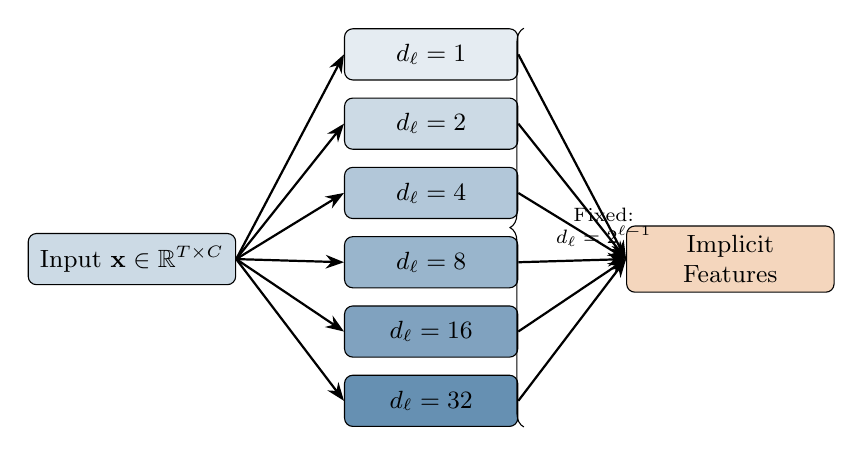
\begin{tikzpicture}[>=Stealth, font=\small,
      box/.style={draw, rounded corners=3pt, minimum width=1.6cm,
                  minimum height=0.65cm, align=center, fill=white},
      dilbox/.style={draw, rounded corners=3pt, minimum width=2.2cm,
                     minimum height=0.65cm, align=center},
      arr/.style={->, thick}
    ]
    \node[box, fill=approachblue!20, text width=2.4cm] (inp) at (0,0)
          {Input $\xv \in \RR^{T \times C}$};

    \foreach \d/\i/\shade in {1/1/10, 2/2/20, 4/3/30, 8/4/40, 16/5/50, 32/6/60}{
      \node[dilbox, fill=approachblue!\shade] (d\i) at (3.8, {2.6-(\i-1)*0.88})
            {$d_\ell=\d$};
    }

    \node[box, fill=accentorange!30, text width=2.4cm] (out) at (7.6,0)
          {Implicit Features};

    \foreach \i in {1,...,6}{
      \draw[arr] (inp.east) -- (d\i.west);
      \draw[arr] (d\i.east) -- (out.west);
    }

    \draw[decorate, decoration={brace, amplitude=5pt, mirror}]
      ([xshift=2pt]d1.north east) -- ([xshift=2pt]d6.south east)
      node[midway, right=8pt, align=center, font=\scriptsize]
        {Fixed:\\$d_\ell=2^{\ell-1}$};
  \end{tikzpicture}
  \caption{Current SSSDTCN implicit module: six dilated causal convolution
           layers with a fixed exponential dilation schedule.}
  \label{fig:current}
\end{figure}

\newpage

%=============================================================================
\section{Approach I: Learnable Soft Dilation Parameters}
%=============================================================================

Inspired by \textbf{Deformable Convolutional Networks}~\citep{dai2017deformable},
which showed that sampling offsets in convolutional kernels can be learned from
data rather than fixed on a regular grid, this approach extends the same
principle to the temporal dilation axis. Each layer $\ell$ is assigned an
unconstrained trainable scalar $\lambda_\ell \in \mathbb{R}$; the effective
dilation factor is $d_\ell = \exp(\lambda_\ell)$, which is always positive and
differentiable. For non-integer $d_\ell$, the convolution uses linear
interpolation between adjacent time steps, so the gradient flows back to
$\lambda_\ell$ via the chain rule. The key to adaptivity is that
$\{\lambda_\ell\}$ are jointly optimised with all other model weights during
end-to-end training, so the dilation schedule converges to the values that best
explain the training data---rather than the values a human engineer pre-selected.

\medskip

\noindent\textbf{Core equations.}
\begin{align}
  d_\ell &= \exp(\lambda_\ell), \label{eq:softd}\\
  (\xv \star_{d_\ell} \wv)[t]
    &= \sum_{i=0}^{k-1} \wv[i]\cdot
       \underbrace{(1-\{d_\ell i\})\,\xv[\lfloor t-d_\ell i\rfloor]
                  +\{d_\ell i\}\,\xv[\lceil t-d_\ell i\rceil]}_{
                  \text{linear interpolation}}, \label{eq:softconv}\\
  \mathcal{L} &= \mathcal{L}_{\text{impute}}
               - \beta\!\sum_{\ell<\ell'}\!|d_\ell - d_{\ell'}|,
               \label{eq:divreg}
\end{align}
where $\{u\}$ is the fractional part of $u$ and the diversity term
\cref{eq:divreg} (weight $\beta>0$) prevents all layers from collapsing to the
same dilation value.

\begin{figure}[H]
  \centering
  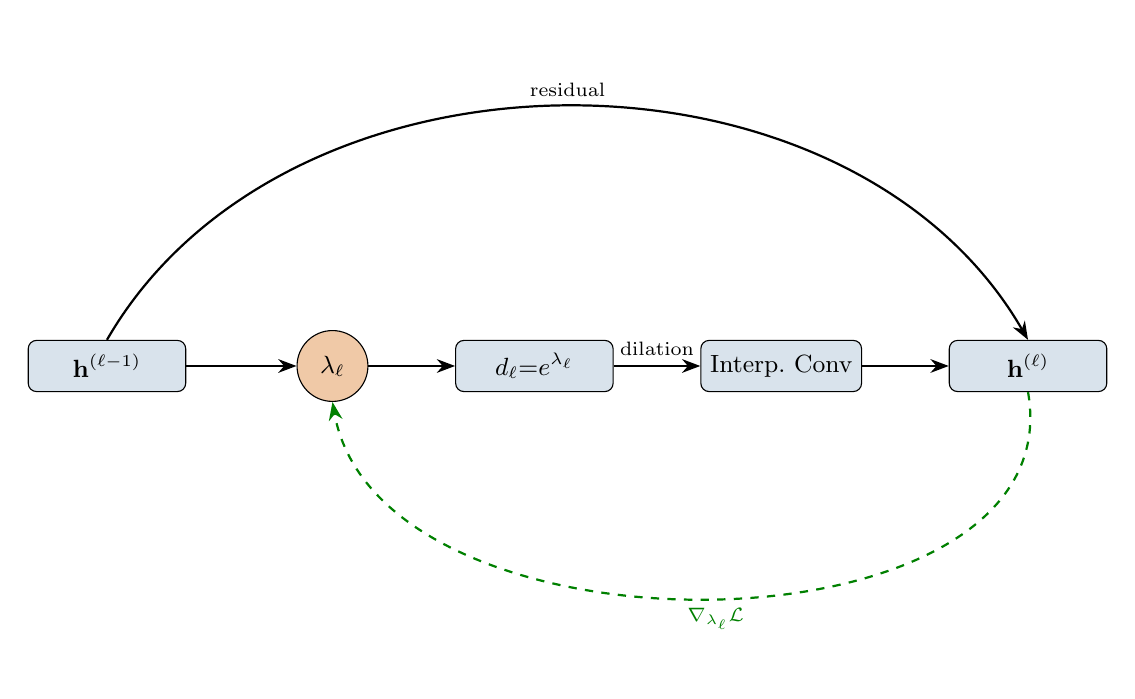
\begin{tikzpicture}[>=Stealth, font=\small,
      box/.style={draw, rounded corners=3pt, fill=approachblue!15,
                  minimum width=2.0cm, minimum height=0.65cm, align=center},
      param/.style={draw, circle, fill=accentorange!40, minimum size=0.9cm,
                    font=\small},
      arr/.style={->, thick}
    ]
    \node[box] (h0) {$\hv^{(\ell-1)}$};
    \node[param, right=1.4cm of h0] (lam) {$\lambda_\ell$};
    \node[box, right=1.1cm of lam] (exp) {$d_\ell{=}e^{\lambda_\ell}$};
    \node[box, right=1.1cm of exp] (conv) {Interp.\ Conv};
    \node[box, right=1.1cm of conv] (out) {$\hv^{(\ell)}$};

    \draw[arr] (h0) -- (lam);
    \draw[arr] (lam) -- (exp);
    \draw[arr] (exp) -- node[above, font=\scriptsize]{dilation} (conv);
    \draw[arr] (conv) -- (out);
    \draw[arr] (h0.north) to[out=60, in=120]
               node[above, font=\scriptsize]{residual} (out.north);
    \draw[->, dashed, color=mathgreen, thick]
      (out.south) to[out=-80, in=-80]
      node[below, font=\scriptsize\color{mathgreen}]{$\nabla_{\lambda_\ell}\mathcal{L}$}
      (lam.south);
  \end{tikzpicture}
  \caption{Approach~I: the dilation $d_\ell=e^{\lambda_\ell}$ is a trainable
           scalar. Gradients (green dashed) flow through the interpolated
           convolution and update $\lambda_\ell$ end-to-end.}
  \label{fig:approach1}
\end{figure}

\clearpage
%=============================================================================
\section{Approach II: Input-Conditioned Selective Kernel Dilation}
%=============================================================================

This approach adapts the idea of \textbf{Selective Kernel Networks
(SKNet)}~\citep{li2019selective} and \textbf{Squeeze-and-Excitation Networks
(SENet)}~\citep{hu2018squeeze} to the temporal dilation setting. SKNet showed
that, for a given input, a network can dynamically choose which kernel size to
emphasise by routing features through a lightweight attention module. Here, $K$
parallel dilated convolutions with distinct fixed candidate rates
$D=\{d^{(1)},\ldots,d^{(K)}\}$ are applied to the same input simultaneously.
Their outputs are aggregated, globally average-pooled into a compact descriptor,
and passed through two fully-connected layers to produce per-channel soft
selection weights $\alpha^{(j)} \in [0,1]^H$ for each branch. The final output
is the weighted sum of all branch outputs. Adaptivity arises because the
selection weights are \emph{conditioned on the current input}: different input
segments or samples yield different $\alpha^{(j)}$, so the effective dilation
shifts automatically to match the dominant temporal scale of each input.

\medskip

\noindent\textbf{Core equations.}
\begin{align}
  \tilde{\hv}^{(j)} &= \mathrm{BN}\!\left(\mathrm{Conv}_{d^{(j)}}(\hv^{(\ell-1)})\right),
    \quad j=1,\ldots,K, \label{eq:sk_split}\\
  \mathbf{s} &= \mathrm{AvgPool}\!\left(\textstyle\sum_j \tilde{\hv}^{(j)}\right)\in\mathbb{R}^H,
    \label{eq:sk_squeeze}\\
  \boldsymbol{\alpha}^{(j)} &= \operatorname{softmax}_j\!\left(\mathbf{W}_2^{(j)}
    \mathrm{ReLU}(\mathbf{W}_1 \mathbf{s})\right) \in [0,1]^H,
    \label{eq:sk_attn}\\
  \hv^{(\ell)} &= \sum_{j=1}^{K} \boldsymbol{\alpha}^{(j)} \odot \tilde{\hv}^{(j)}.
    \label{eq:sk_out}
\end{align}
The input-level effective dilation at time $t$ is interpretable as
$d_\ell^{\text{eff}}(t)=\sum_j \bar{\alpha}^{(j)}(t)\cdot d^{(j)}$, where
$\bar{\alpha}^{(j)}(t)$ is the channel-mean weight.

\begin{figure}[H]
  \centering
  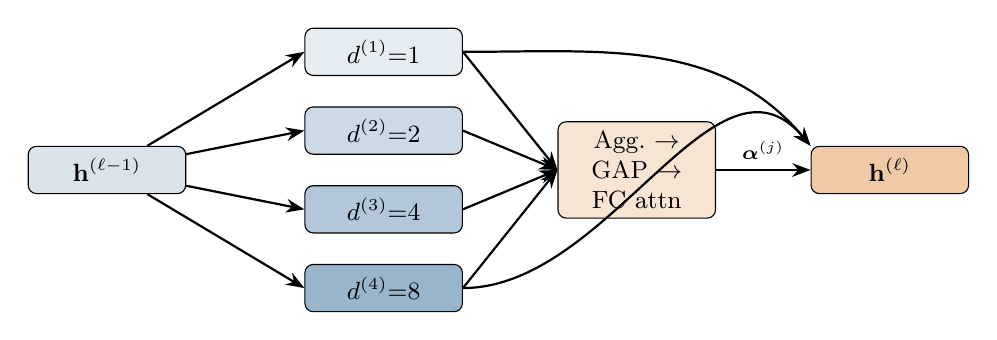
\begin{tikzpicture}[>=Stealth, font=\small,
      box/.style={draw, rounded corners=3pt, minimum width=2.0cm,
                  minimum height=0.60cm, align=center},
      arr/.style={->, thick}
    ]
    \node[box, fill=approachblue!15] (h) {$\hv^{(\ell-1)}$};

    \node[box, fill=approachblue!10, right=1.5cm of h, yshift= 1.5cm] (b1)
          {$d^{(1)}{=}1$};
    \node[box, fill=approachblue!20, right=1.5cm of h, yshift= 0.5cm] (b2)
          {$d^{(2)}{=}2$};
    \node[box, fill=approachblue!30, right=1.5cm of h, yshift=-0.5cm] (b3)
          {$d^{(3)}{=}4$};
    \node[box, fill=approachblue!40, right=1.5cm of h, yshift=-1.5cm] (b4)
          {$d^{(4)}{=}8$};

    \foreach \b in {b1,b2,b3,b4}{ \draw[arr] (h) -- (\b.west); }

    \node[box, fill=accentorange!20, right=1.2cm of b2, yshift=-0.5cm] (agg)
          {Agg.\ $\rightarrow$\\GAP $\rightarrow$\\FC attn};
    \foreach \b in {b1,b2,b3,b4}{ \draw[arr] (\b.east) -- (agg.west); }

    \node[box, fill=accentorange!40, right=1.2cm of agg] (out)
          {$\hv^{(\ell)}$};
    \draw[arr] (agg) -- node[above, font=\scriptsize]{$\boldsymbol{\alpha}^{(j)}$} (out);
    \foreach \b in {b1,b4}{
      \draw[arr] (\b.east) to[out=0, in=130] (out.north west);
    }
  \end{tikzpicture}
  \caption{Approach~II: four parallel branches with different dilation rates.
           The squeeze-and-excitation block produces input-conditioned per-channel
           attention weights that recombine the branch outputs.}
  \label{fig:approach2}
\end{figure}

\clearpage
%=============================================================================
\section{Approach III: Differentiable Architecture Search for Dilation Rates}
%=============================================================================

\textbf{DARTS (Differentiable ARchiTecture Search)}~\citep{liu2019darts}
introduced continuous relaxation of discrete architecture choices via a
\emph{mixed operation}: instead of committing to one operation, a weighted
mixture of all candidate operations is used during search, with mixture weights
jointly optimised via gradient descent. Translated to the dilation setting,
each layer $\ell$ maintains a real-valued architecture parameter vector
$\boldsymbol{\alpha}_\ell \in \mathbb{R}^K$ over $K$ candidate dilations. During
the search phase, the layer computes a softmax-weighted mixture of all $K$
dilated convolutions; after search, the candidate with the highest weight is
selected and the final model is retrained from scratch with those discrete rates.
Adaptivity is dataset-level: the architecture search explores a rich dilation
space $D=\{1,2,3,4,6,8,12,16,24,32\}$ and converges to the schedule that
minimises validation loss---no human choice required.

\medskip

\noindent\textbf{Core equations.}
\begin{align}
  \bar{o}^{(\ell)}(\hv) &= \sum_{j=1}^{K}
    \frac{\exp(\alpha_\ell^{(j)})}{\sum_{j'}\exp(\alpha_\ell^{(j')})}
    \cdot\mathrm{Conv}_{d^{(j)}}(\hv), \label{eq:darts_mix}\\
  \thetav &\leftarrow \thetav - \eta_\theta
    \nabla_{\thetav}\mathcal{L}_{\text{train}}(\thetav,\alphav), \label{eq:darts_w}\\
  \alphav &\leftarrow \alphav - \eta_\alpha
    \nabla_{\alphav}\mathcal{L}_{\text{val}}(\thetav,\alphav), \label{eq:darts_a}\\
  d_\ell^* &= d^{(\hat{j}_\ell)}, \quad
    \hat{j}_\ell = \arg\max_j\,\alpha_\ell^{(j)}. \label{eq:darts_disc}
\end{align}
Equations~\cref{eq:darts_w,eq:darts_a} are the alternating gradient steps of
the bi-level optimisation; \cref{eq:darts_disc} is the final discretisation.

\begin{figure}[H]
  \centering
  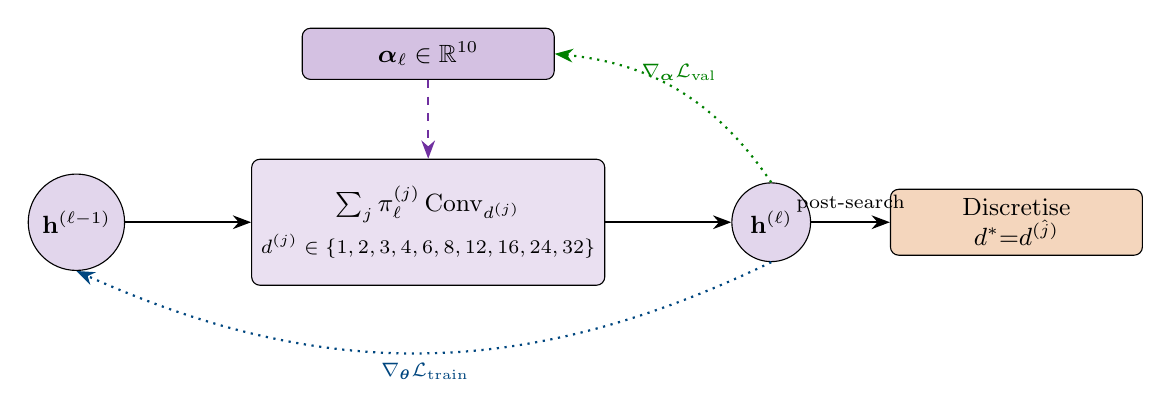
\begin{tikzpicture}[>=Stealth, font=\small,
      snode/.style={draw, circle, fill=approachpurple!20, minimum size=1.0cm},
      ebox/.style={draw, rounded corners=3pt, fill=approachpurple!15,
                   minimum width=3.2cm, minimum height=0.65cm, align=center},
      arr/.style={->, thick}
    ]
    \node[snode] (n0) at (0,0) {$\hv^{(\ell-1)}$};

    \node[ebox, minimum height=1.6cm, right=1.6cm of n0] (mix)
      {$\sum_j \pi_\ell^{(j)}\,\mathrm{Conv}_{d^{(j)}}$\\[4pt]
       \scriptsize $d^{(j)}\in\{1,2,3,4,6,8,12,16,24,32\}$};

    \node[snode, right=1.6cm of mix] (n1) {$\hv^{(\ell)}$};

    \draw[arr] (n0) -- (mix);
    \draw[arr] (mix) -- (n1);

    \node[ebox, fill=approachpurple!30, above=1.0cm of mix] (alpha)
          {$\boldsymbol{\alpha}_\ell\in\mathbb{R}^{10}$};
    \draw[->, dashed, thick, color=approachpurple] (alpha.south) -- (mix.north);

    \draw[->, dotted, thick, color=mathgreen, bend right=25]
      (n1.north) to node[above, font=\scriptsize\color{mathgreen}]
      {$\nabla_{\alphav}\mathcal{L}_{\text{val}}$} (alpha.east);
    \draw[->, dotted, thick, color=approachblue, bend left=25]
      (n1.south) to node[below, font=\scriptsize\color{approachblue}]
      {$\nabla_{\thetav}\mathcal{L}_{\text{train}}$} (n0.south);

    \node[ebox, fill=accentorange!30, right=1.0cm of n1] (disc)
          {Discretise\\$d^*{=}d^{(\hat{j})}$};
    \draw[->, thick] (n1) -- (disc)
      node[midway, above, font=\scriptsize]{post-search};
  \end{tikzpicture}
  \caption{Approach~III: DARTS mixed operation. During search all candidate
           dilations are active (weighted by $\pi_\ell^{(j)}$). After search
           the best-scoring dilation is selected (orange box).}
  \label{fig:approach3}
\end{figure}

\clearpage
%=============================================================================
\section{Approach IV: Frequency-Spectral Guided Adaptive Dilation}
%=============================================================================

\textbf{TimesNet}~\citep{wu2023timesnet} and
\textbf{FEDformer}~\citep{zhou2022fedformer} demonstrated that industrial and
meteorological time series carry strong periodicity, and that aligning model
structure with dominant periods substantially improves performance. This
approach applies the same insight directly to dilation-rate setting: the Fast
Fourier Transform is applied to the training data to locate the $L$ dominant
frequency components, each is converted to a period $P_\ell = T / f_\ell$, and
the dilation for layer $\ell$ is then set so that the kernel's sampling stride
matches one full period---$d_\ell = \lfloor P_\ell/(k-1)\rfloor$. No
additional trainable parameters are introduced; the entire calibration runs
once as an offline pre-processing step, and the resulting dilation schedule is
automatically customised to each dataset's physical periodicity.

\medskip

\noindent\textbf{Core equations.}
\begin{align}
  A_f &= \frac{1}{C}\sum_{c=1}^C \bigl|\FFT(\xv[c,:])[f]\bigr|,
    \quad f=1,\ldots,\lfloor T/2\rfloor, \label{eq:fft}\\
  \{f_1,\ldots,f_L\} &= \TopK\!\left(\{A_f\},\,L\right), \label{eq:topk}\\
  P_\ell &= \left\lfloor T / f_\ell \right\rceil, \label{eq:period}\\
  d_\ell &= \max\!\left(1,\,\left\lfloor P_\ell/(k-1)\right\rceil\right). \label{eq:freqdil}
\end{align}

\begin{figure}[H]
  \centering
  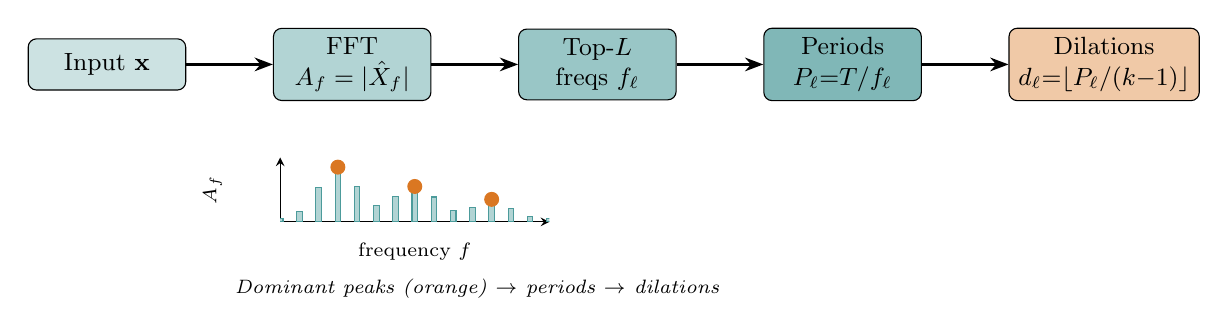
\begin{tikzpicture}[>=Stealth, font=\small,
      box/.style={draw, rounded corners=3pt, minimum width=2.0cm,
                  minimum height=0.65cm, align=center, fill=approachteal!20},
      arr/.style={->, thick}
    ]
    \node[box] (inp) {Input $\xv$};
    \node[box, fill=approachteal!30, right=1.1cm of inp] (fft)
          {FFT\\$A_f=|\hat{X}_f|$};
    \node[box, fill=approachteal!40, right=1.1cm of fft] (topk)
          {Top-$L$\\freqs $f_\ell$};
    \node[box, fill=approachteal!50, right=1.1cm of topk] (per)
          {Periods\\$P_\ell{=}T/f_\ell$};
    \node[box, fill=accentorange!40, right=1.1cm of per] (dil)
          {Dilations\\$d_\ell{=}\lfloor P_\ell/(k{-}1)\rfloor$};

    \draw[arr] (inp) -- (fft);
    \draw[arr] (fft) -- (topk);
    \draw[arr] (topk) -- (per);
    \draw[arr] (per) -- (dil);

    % Small spectrum sketch below
    \begin{scope}[shift={(2.2,-2.0)}]
      \begin{axis}[
          width=5cm, height=2.4cm,
          xtick=\empty, ytick=\empty,
          axis lines=left,
          xlabel={\scriptsize frequency $f$},
          ylabel={\scriptsize $A_f$},
          x label style={font=\tiny, at={(axis description cs:0.5,-0.18)}, anchor=north},
          y label style={font=\tiny, at={(axis description cs:-0.18,0.5)}, anchor=south},
          ymin=0, ymax=1.0,
        ]
        \addplot[fill=approachteal!30, draw=approachteal!70, ybar, bar width=2pt,
                 samples at={1,2,...,15}]
          {0.05+0.8*exp(-0.5*(x-4)^2)+0.5*exp(-0.4*(x-8)^2)
               +0.3*exp(-0.6*(x-12)^2)};
        \addplot[mark=*, mark size=2.5pt, color=accentorange, only marks]
          coordinates{(4,0.85) (8,0.55) (12,0.35)};
      \end{axis}
      \node[font=\scriptsize\itshape, below=0pt] at (2.5,-0.6)
            {Dominant peaks (orange) $\rightarrow$ periods $\rightarrow$ dilations};
    \end{scope}
  \end{tikzpicture}
  \caption{Approach~IV: the FFT magnitude spectrum is computed once from the
           training set; the $L$ largest peaks (orange dots) determine periods
           $P_\ell$, which are mapped to dilation rates $d_\ell$.}
  \label{fig:approach4}
\end{figure}

\clearpage
%=============================================================================
\section{Approach V: Temporal Self-Attention Guided Dynamic Dilation}
%=============================================================================

\textbf{Dynamic Convolution}~\citep{chen2020dynamic} showed that conditioning
convolution kernels on the current input context---rather than using fixed
weights---substantially increases representational capacity.
\textbf{Non-local Means}~\citep{wang2018nonlocal} similarly showed the benefit
of using position-level attention to identify the most informative temporal
offsets. Combining these ideas, this approach inserts a lightweight temporal
self-attention module before the convolution: query and key projections are
applied to the hidden state, producing a per-position attention score
$a_{t,\delta}$ for each candidate offset $\delta$. The expected offset
$\bar{d}_t = \sum_\delta \delta\,a_{t,\delta}$ gives a continuous,
position-level effective dilation that varies \emph{within a single sequence}:
high-frequency regions concentrate weight on small offsets (fine scale), while
smoother or longer-range regions concentrate weight on large offsets (coarse
scale). A multiplicative gate then modulates the base dilation $d_\ell^{(0)}$
of the original layer by this context-dependent factor.

\medskip

\noindent\textbf{Core equations.}
\begin{align}
  e_{t,\delta} &= \frac{\mathbf{q}_t^\top \mathbf{k}_{t-\delta}}{\sqrt{d_k}},
    \quad
    a_{t,\delta} = \frac{\exp(e_{t,\delta})}{\sum_{\delta'}\exp(e_{t,\delta'})},
    \label{eq:attn}\\
  \bar{d}_t &= \sum_{\delta=0}^{T_{\max}} \delta\cdot a_{t,\delta},
    \label{eq:effd}\\
  \tilde{d}_{t,\ell} &= d_\ell^{(0)}\cdot
    2\,\sigmoid\!\left(\mathbf{w}_s^\top\hv^{(\ell-1)}[:,t]+b_s\right),
    \label{eq:dyngate}
\end{align}
where \cref{eq:dyngate} bounds the adapted dilation in $[0, 2d_\ell^{(0)}]$.

\begin{figure}[H]
  \centering
  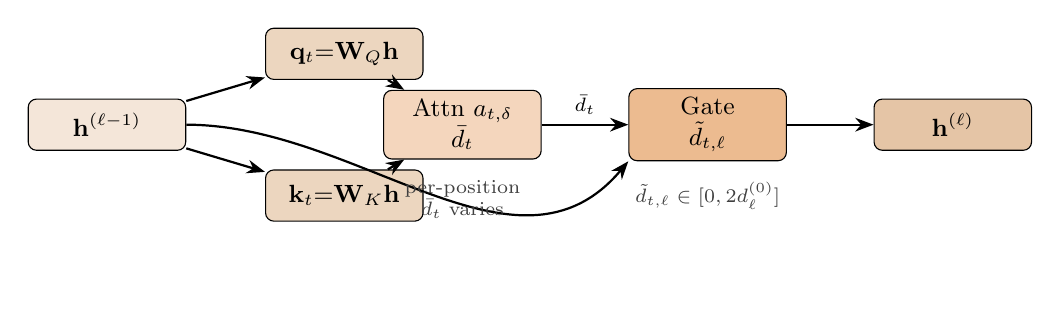
\begin{tikzpicture}[>=Stealth, font=\small,
      box/.style={draw, rounded corners=3pt, minimum width=2.0cm,
                  minimum height=0.65cm, align=center, fill=approachorange!15},
      arr/.style={->, thick}
    ]
    \node[box] (h0) {$\hv^{(\ell-1)}$};

    \node[box, fill=approachorange!25, right=1.0cm of h0, yshift= 0.9cm]
      (q) {$\mathbf{q}_t{=}\mathbf{W}_Q\hv$};
    \node[box, fill=approachorange!25, right=1.0cm of h0, yshift=-0.9cm]
      (k) {$\mathbf{k}_t{=}\mathbf{W}_K\hv$};

    \draw[arr] (h0) -- (q);
    \draw[arr] (h0) -- (k);

    \node[box, fill=accentorange!30, right=2.5cm of h0] (attn)
          {Attn $a_{t,\delta}$\\$\bar{d}_t$};
    \draw[arr] (q) -- (attn);
    \draw[arr] (k) -- (attn);

    \node[box, fill=accentorange!50, right=1.1cm of attn] (gate)
          {Gate\\$\tilde{d}_{t,\ell}$};
    \draw[arr] (attn) -- (gate)
      node[midway, above, font=\scriptsize]{$\bar{d}_t$};
    \draw[arr] (h0.east) to[out=0, in=-130] (gate.south west);

    \node[box, fill=approachorange!35, right=1.1cm of gate] (out)
          {$\hv^{(\ell)}$};
    \draw[arr] (gate) -- (out);

    \node[font=\scriptsize, below=4pt of attn, text=darkgray, align=center]
          {per-position\\$\bar{d}_t$ varies};
    \node[font=\scriptsize, below=4pt of gate, text=darkgray, align=center]
          {$\tilde{d}_{t,\ell}\in[0,2d^{(0)}_\ell]$};
  \end{tikzpicture}
  \caption{Approach~V: a self-attention module computes a per-position expected
           offset $\bar{d}_t$; a sigmoid gate (right) scales the base dilation
           $d_\ell^{(0)}$ by a context-dependent factor, producing a fully
           position-adaptive effective dilation.}
  \label{fig:approach5}
\end{figure}

\clearpage
%=============================================================================
\section{Comparative Discussion}
%=============================================================================

\Cref{tab:comparison} summarises the five approaches along key design
dimensions. The recommended starting point is a hybrid of Approaches~IV and~I:
use the spectral calibration (\cref{eq:freqdil}) to set the initial
$\lambda_\ell^{(0)}=\log(d_\ell^{\text{spectral}})$, then fine-tune with
learnable soft dilations. This combines physics-guided initialisation with
gradient-based refinement at minimal implementation cost.

\vspace{6pt}

\begin{table}[H]
  \centering
  \caption{Comparison of adaptive dilation approaches.}
  \label{tab:comparison}
  \setlength{\tabcolsep}{5pt}
  \renewcommand{\arraystretch}{1.25}
  \begin{tabular}{@{}lccccl@{}}
    \toprule
    \textbf{Approach} & \textbf{Extra params} & \textbf{Adapt.\ level}
      & \textbf{Search?} & \textbf{Infer.\ cost} & \textbf{Key reference} \\
    \midrule
    Fixed (baseline)   & 0            & ---          & No       & $\mathcal{O}(LC)$    & --- \\
    I.\ Soft dilation  & $L$ scalars  & Global       & No       & $\mathcal{O}(LC)$    & \cite{dai2017deformable}\\
    II.\ SKNet fusion  & $O(KH^2)$    & Per-sample   & No       & $\mathcal{O}(KLC)$   & \cite{li2019selective}\\
    III.\ DARTS        & $LK$ (search)& Global       & Yes      & $\mathcal{O}(LC)$    & \cite{liu2019darts}\\
    IV.\ Spectral      & 0            & Global       & No       & $\mathcal{O}(LC)$    & \cite{wu2023timesnet}\\
    V.\ Attn-guided    & $O(Hd_k L)$  & Per-position & No       & $\mathcal{O}(LCT)$   & \cite{chen2020dynamic}\\
    \bottomrule
  \end{tabular}
\end{table}

%=============================================================================
\bibliographystyle{plainnat}
\begin{thebibliography}{99}

\bibitem[Chen et al.(2020)]{chen2020dynamic}
Chen, Y., Dai, X., Liu, M., Chen, D., Yuan, L., \& Liu, Z. (2020).
Dynamic convolution: Attention over convolution kernels.
\textit{CVPR}, pp.\ 11030--11039.

\bibitem[Dai et al.(2017)]{dai2017deformable}
Dai, J., Qi, H., Xiong, Y., Li, Y., Zhang, G., Hu, H., \& Wei, Y. (2017).
Deformable convolutional networks.
\textit{ICCV}, pp.\ 764--773.

\bibitem[Hu et al.(2018)]{hu2018squeeze}
Hu, J., Shen, L., \& Sun, G. (2018).
Squeeze-and-excitation networks.
\textit{CVPR}, pp.\ 7132--7141.

\bibitem[Li et al.(2019)]{li2019selective}
Li, X., Wang, W., Hu, X., \& Yang, J. (2019).
Selective kernel networks.
\textit{CVPR}, pp.\ 510--519.

\bibitem[Liu et al.(2019)]{liu2019darts}
Liu, H., Simonyan, K., \& Yang, Y. (2019).
DARTS: Differentiable architecture search.
\textit{ICLR}.

\bibitem[Wang et al.(2018)]{wang2018nonlocal}
Wang, X., Girshick, R., Gupta, A., \& He, K. (2018).
Non-local neural networks.
\textit{CVPR}, pp.\ 7794--7803.

\bibitem[Wu et al.(2023)]{wu2023timesnet}
Wu, H., Hu, T., Liu, Y., Zhou, H., Wang, J., \& Long, M. (2023).
TimesNet: Temporal 2D-variation modeling for general time series analysis.
\textit{ICLR}.

\bibitem[Zhou et al.(2022)]{zhou2022fedformer}
Zhou, T., Ma, Z., Wen, Q., Wang, X., Sun, L., \& Jin, R. (2022).
FEDformer: Frequency enhanced decomposed transformer for long-term series
forecasting.
\textit{ICML}, pp.\ 27268--27286.

\end{thebibliography}

\end{document}
